
\chapter{维基百科用户参与知识协同的动机因素模型}
\label{cha:motivation}



越来越多的学者已经注意到维基百科的日益流行及其取得的巨大成功。维基百科
社区以一种前所未有的运作方式吸引了大量的志愿者自愿为其撰写内容,并为此
付出了巨大的精力,投入了大量的时间。不论是维基百科的研究者,还是社区的
运营者都自然地关注一个问题,到底是什么因素促使如此众多的人员参与到这项
庞大的计划中,并创造出传统方式难于匹敌的数量的内容?

当前已经有一些学者针对维基百科用户参与社区的动机因素进行了研究,并取得
了一定的成果。但是,这些成果主要是关于为何维基用户参与知识共享的动机的
研究。知识共享是以共享为目的,以知识的传递和流动为表象,达到知识的发送
方和接收方共同拥有同一知识的结果。在维基百科社区中,知识共享主要发生于
条目的作者和读者之间。条目的作者拥有同条目主题相关的知识,并将这些知识
按照一定的格式撰写出来。当读者对某种知识有需求的时候,通过阅读条目
的内容从中吸收和掌握知识,进而完成编写者和读者之间的知识共享。相对作者
与读者之间的知识
共享关系来说,条目作者之间的关系主要是协同关系。每个作者都只拥有关于某
个条目的一部分知识,个体的力量不足以完成这个条目的编辑工作,必须依靠协
同的方式来弥补知识的缺口,共同完成条目的撰写。
协同过程中存在一定的知识共享,但是知识共享不是协同的主要目的,它只是协
同过程中所连带产生的结果。知识协同最终的目的是为了完成条目。

个人将自身的知识同其他人共享,一般来讲除了纯粹的利他以外,往往是出于以下几个目的:1)为了获得
物质奖励;2)为了获得其他非物质的收益,如名誉,其他人的认同和赞扬
等;3)期望与其他人互惠互利,在将来一旦有知识需求的时候能从他人那里获
得帮助\cite{Zhugea}。显然,这几种因素均不能完全反应维基百科用户参与知识协同的动机。首先,维
基百科并不能给用户带来现实的或是潜在的物质收益,用户的参与完全是义务的。其次,根据维基基金会所
作的调查,在所有可能的用户参与维基百科的动机因素中,赢得在社区中的声誉
处于最后一位,大部分用户都不认为这是他们参与到维基百科中的原因
\cite{Glott2009}。Bryant等也指出,协同的本质特征决定了用户几乎不可能通
过协同来获得声誉\cite{1099205}。最
后,在维基百科社区中确实存在一定程度的互惠互利现象,协同双方在协同过程
中满足各自的知识需求。但是,对于相当一部
分用户来说,尤其是领导者和领域专家,互惠互利并不能解释他们参与知识协同
的动机。考虑到这两类用户的知识投入和所获得的他人的知识投入极度的不平
衡,可以认为这两类用户并不指望从其他用户那里获得同自身的投入同等程度的
回报。基于以上原因,目前关于对个人参与虚拟实践社区的动机因素的研究并不
能完全用来解释个体间知识协同的动机。因此,有必要对各种动机因素进行分析
和梳理,构建一个适合于研究个体间知识协同的动机因素模型。

在之前的章节中已经定义了维基百科社区中的知识协同,即对所有条目内容所做
的编辑工作,包括新增内容,删除内容,修改内容等。这些协同行为背后的驱动
力量就是动机。个体的行为往往同时受到多种动机的影响,同时在不同阶段起作
用的动机也不同。更为复杂的是,动机往往易受到外界因素的影响,呈现为增强
或者减弱的趋势。这就需要动机模型不但要反映出各种动机对行为的影响,同时
要考虑时间和外部因素对动机强度的影响,反应各个动机因素间的相互作用。

现有的研究已经提出了很多影响个体行为的动机因素。这些动机因素大致可以分
为两种类型:个体层次的动机因素因素和群体层次的动机因素因素。个体因素强调个体固有的感受和需要,即使
个体处于一个“独立”的环境下,个体因素仍然可以起作用,促使其从事某种行
为。人际因素则存在于个体之间的互动过程中,是其他人的行为加于个体自身的感受和
需要。在知识协同过程中,个体层次的动机因素和群体层次的动机因素同时起作
用,共同影响了个体的
行为。

\section{个体层次的动机因素}
\label{sec:individual-factor}

\subsection{利他主义}
\label{sec:altruism}

利他主义是一种纯粹的、只希望施惠于他人而不谋求从中取得任何收益或者改进自身
状态的动机因素。它是一种人类内在的本质特征,Dixon认为人们天生就喜欢帮助
他人。利他主义认为关注他人的利益应该胜于关心自身的利益。绝大部分参与社区的用户本身并不能从社区中
获得明显的物质回报,(Rachlin, 2002)认为利他主义是解释用户行为可能的因
素之一。在开源社区,在内容贡献社区,利他主义的重要作用都得到了验证\cite{oreg2008exploring}。
Kollock等发现用户参与虚拟社区并义
务共享其知识是因为他们感到帮助他人解决有挑战性的问题很有趣,并且帮助别
人的感觉很好\cite{Smith1999}。kuznetsov认为维基百科中绝大部分活动都可以归结于利他主义
\cite{kuznetsov2006motivations}。由于维基技术的应用压制了个体获得
声誉和认同的需求,因此那些“自私”的人会自动选择不参与社区\cite{4076406}。在维基百
科中,知识协同的最终目标是完成一个条目的创作,个体自身并不能从协同中得
到对其劳动的补偿。但是,个体在利他主义的驱动下,愿意同他人一起完成条
目的编辑工作,因此,利他主义是个人参与知识协同的一个重要动机。

\subsection{感知到的意义}
\label{sec:sense-of-meaning}

感知到的意义(sense of meaningfulness)是个体的一种感知。个体意识到自
己所从事的工作或是追寻的目标是有意义、有价值的,即使投入大量时间和精力
也是值得的。这种感知形成了个体的内
部推动力量,促使个体努力达成预定目标。维基百科的目标是“包含人类所有领域
的知识”,并且“始终保持自由”,可以任意地“被复制,修改和再发布”。绝
大多数维基人都认同这个目标,并且认为他们的工作会“改变
世界”,使更多的人能“自由地访问信息“。

\subsection{自我决定}
\label{sec:self-determination}

自我决定(Self determination)也是一种个体的感知状态。个体意识到自己有
权利决定是否要从事某项工作或者完成某种任务,并且这种选择不受任何外部力
量的影响。Pintrich等认为自我决定理论是如今的动机理论中最全面的、广受实
践检验过的理论。自我决定理论的应用范围非常广泛,近年来在对
在线社区的研究方面更是取得很多的成果。自我决定理论认为人有三种基本需
求:自主性、胜任感和归属感。自主性是指个体感受到能够掌控周围
的环境、事件的进程以及资源的获取的分配;胜任感是指个体认为自己有足够
的能力能够胜任某种工作或者任务;归属感是指个体能够感受到来自他人的关
心。当着三种基本需求得到满足时,个体的心理满足程度则得到加强。

自我决定理论将个体的动机分为三种类型:无动机、外部动机和内部动机。这三
种动机不是孤立地存在的,而是一个连续统一体。无动机是指个体缺乏参与活动
的意图,完全没有自我决定的因素;随着动机的逐渐增强(大部分是由于外部力
量的介入),个体的行为转为受外部动机的影响。这时一定程度的外部激励会弥
补个体的被强迫感觉,增
强个体的动机;当动机进一步增强,个体完全受自身意愿和兴趣所驱使参与某项
活动是,个体的主要驱动因素转为内部动机;个体不在受到任何外部力量的驱使
和强迫,这时外部激励反而会降低个体的内部动机。

从维基百科社区为用户提供了极大的自由,任何人都可以不受限制地参与
编辑,不论是否在社区注册过;社区中也不存在等级制度限制用户编辑的自由,
用户随时可以退出。这种开放性使得用户的自主性得到了极大的满足。这种开放
性还表现为维基百科欢迎任何类型的贡献而不计较贡献的大小,大到完成整个条
目的编写,小到对错别字的订正。这就是每个参与的用户都能找到适合自身的任
务,并提升其胜任感,并最终激发用户的内部动机,自愿地为社区做出贡献。

\subsection{自我效能}
\label{sec:self-efficacy}

自我效能(self-efficacy)是指一个人在特定情景中从事某种行为并取得预期结
果的能力。班杜拉将自我效能定义为:个体对有效控制自己的生活行为等诸方面
的能力的知觉或信念\cite{}。自我效能在很大程度上指个体自己对自我有关能
力的感觉,既对自己是否能够成功地进行某一成就行为的主观判断。一般来说,
成功的经验会增强个体的自我效能,反复的失败会降低个体的自我效能。

Raban等认为,一个人的才学是其所拥有的最宝贵的个人财富,能够与他人分享
这种这份财富会增强个人的自我意识,尤其是在对方表达谢意和尊敬的时候增强
的程度更为明显\cite{raban2007investigating}。Chan等研究了虚拟社区中的
知识共享行为,发现那些共享者在从他人那里获得了正向的反馈之后自我效能得
到了很大的提升,这种自我增强反过来又进一步促使他们分享更多的知识。
自我效能高的个体比那些自我效能低的个体更愿意参与到相关活动中去,因为他
们相信自己有能力取得预期的效果。相反的,自我效能低的个体常常缺乏参与的
动力,或者不愿意面对可能出现的困难,从而降低了参与的动机。

个体的自我效能主要受到四种因素的影响:个人成就、替代性经验、言语说服和
情绪激发。个体自身的成功经验是影响自我效能的最重要的因素。一旦个体成功
地完成了某项任务,将大大地提升个体对自身能力的信心,激发自身的自我效
能;而失败会使个体对自身能力产生怀疑,进而降低其参与动机。他人的经验对
于个体的自我效能也有很大的影响。通过观察他人的行动判断任务的特点和难
点,从中吸取经验并学习必要的技巧,个体能够显著地改善和提升自身的绩效。
他人对与个体的鼓励和帮助能增强个体的动机。当个体受到他人的激励,树立自身
能够成功完成某项任务的信念是时,个体的自我效能就会相应得到提升。帮助的
形式可能有言语上的激励、直接的指导以及对个体行为绩效的反馈等形式。个体
的情绪和心理状态对于个体对特定任务的判断起到很大的影响。高昂的情绪和积
极的心理状态往往会提升个体对自身能力的判断,激发个体潜能,改善其对参与
的预期结果的判断。负面的情绪,如焦虑等则会降低个体对自身能力的判断、夸
大任务的难度、降低预期收益,最终导致自我效能的较低。

维基百科的用户主要行为就是知识协同。社区为用户提供了多样的手段来克服对
社区的生疏感和对协同的“恐惧感”:既有详尽的使用说明和新手指南,同时又
可以得到资深用户的指导。新用户既可以通关观察自身用户的行为学习社区内的
协同方式,又可以在宽容的气氛中开始尝试协同而不必担心会收到批评和指责。
一旦个体的内容能够在未来的编辑中得以留存,就意味着个人的贡献受到了其他协同者的认可。个
体在协同中既获得了经验,同时也获得了心理上的满足和愉悦,从而提升其自我
效能。而更高的自我效能又提升了用户的参与水平。自我效能感与成就行为是相互促进的,它是用户参与维基百科重要的内部动机因素。

\subsection{自我肯定}
\label{sec:self-esteem}

自我肯定(Self-esteem)又称为自我价值、自尊等,是个体对于自我形象的主
观感觉,这种感觉可以是过分的或不合理的。自我肯定常常同自我效能相混淆。
自我效能是对特定能力的一种判断,而非自我价值的一般性感受。这种特定能力
总是与特定目标相联系的。有些人具备很高的“自我效能”──努力驱动自我,
但是自我肯定的意识却不强。另一方面,有些人可能对自身的价值非常肯定,但
是当遇到某一特定问题时,却缺乏足够的自我效能。

高自我肯定的人对于自身价值的评价很高,但同时又能清楚地认识到自身的缺点
和不足。高自我肯定的人乐于去学习、改进和提高自己,这类人通常表现为性格
外向、很受别人欢迎、工作认真尽责、善于控制情绪并且喜欢各种不同的体验。
而低自我肯定的人
表现为对自己的不满和自我否定,不喜欢自己当前的样子,这类人通常表现为性
格沉闷、不擅同人交往、情绪波动大。低自我肯定的人试图努力改变当前自身的
形象,为此需要不断地投入到某种活动中来证明自己;高自我肯定的
人通常倾向于维持这种良好的自我感觉,因此也乐于参与到活动中获得自身形象进一步的
提升。这就成
了个体参与某项任务的基本动机。

维基百科为用户强化其自我肯定的意识提供了良好的媒介。它的独特之处就在于
个体可以通过适当的策略尽量提升自身肯定,同时又不必承担不被别人所认同的
风险。
这是因为其他人的冷淡和忽视可以被贡献者自身直接理解为认同。不论条目的内容是否充
实,也不论文字是否有错误,只要没人提出或者修正,对于作者本身来说就是好的。同
时,各个条目之间又是平等的,即使是很小的条目,作者也会获得等量的参与感
和满足感。这使
得在维基百科中获得自我肯定极其容易。Timme等指出在维基百科中提升自我肯
定的最佳策略就是撰写那些受众较小的条目,获得最大收益的同时还尽量降低了
风险。

Tice (1993)认为低自我效能的人因为没有什
么负担,故愿意采用那些风险较大但是见效较快的行动来快速改进自身的形象。
而高自我肯定的人为了维持自身的形象,因此对于参与活动往往持稳健和保守的
态度,力求凡是做到尽善尽美。因此尽管高自我肯定的人和低自我肯定的人都有
很强的参与维基百科的动机,但是他们在社区中的表现是不一致的。高自我肯定
的人会重视条目的质量和内容的编排,努力编写完善的条目,而低自我肯定的人
则是“重在参与”,贡献的内容往往质量不高,主题生僻。

\subsection{成就动机}
\label{sec:achievement}
成就动机(achivement motivation),是个体追求自认为重要的有价值的工作,并
使之达到完美状态的动机。在这种动机的驱动下,个体愿意从事这项工作,并尽
力取得成功。Clark等将成就动机定义为对优秀标准的竞争或个体设定、实现个
体目标的愿望。
阿特金森认为个体的动机水平依赖于3大因素:成功诱因值,即对实现目标的价
值判断;成功的可能性大小以及成就需要,即主体追求成功的动机强度。这3个
因素发生综合影响,决定了个体的主观倾向和投入程度。

麦克利兰的成就动机理论进一步揭示了成就动机如何影响人的行为。个体记忆中存在着与成就相联系的愉快经验,
当情境能引起这些愉快经验时,就能激发人的成就动机欲望。个人的成就动机包
括三个方面:成就需要、权利需要和亲和需要。这三种需要在人们需要结构中有
主次之分,作为人们的主需求在满足了以后往往会要示更多更大的满足,拥有
成就者更追求成就,拥有权力者更追求权力、拥有亲情者更追求亲情。同时,成就需要的高低对人的成长和发展起到特别重要的作用,

成就需要是个体设定目标并努力达成目标的需要,个体从中获得优越感和满足感。
个人体自己认为重要或有价值的工作,不但愿意去做,而且会投入大量的时间和
精力,力
求达到完美地步。在这种动机驱使下,个体不是去追求由于成就本身所带来的报
酬,而是谋求把事情做得更好、更有效果。参与维基百科的用户正是在完成协同
任务的过程中,满足个人对于成就的渴望。

权力需要是指个体试图影响或控制他人且不受他人控制的需要。对于权利需求较
高的人来说,对他人施加影响要比工作本身更值得追求。这类人通常偏好于有竞
争性和地位取向的场合。尽管维基用户本质上不存在等级划分,但是一部分用户仍然通过自己的
表现成为了事实上的领导者。领导者的意见和建议对于社区的其他成员具有很大
的影响,他们的价值取向也往往成为某个用户群体的价值取向。特别是当协同实
践出现争议和矛盾时,社区领导者往往会利用自身的地位加以解决,这反过来又
进一步强化了其领导者的优势。

亲和需求是个体希望同其他人建立友好亲密的人际关系的需要。亲和需求促使个
体追求友善,重视人际关系。个体从他人的交往中获得愉悦感。亲和需求是虚拟
实践社区存在和发展的重要保证。在知识协同过程中,只有协同的各方互相尊
重,互相体谅,才能保证协同的顺利开展,取得最大的协同效应。

\section{群体动机}
\label{sec:groupe-motivation}

\subsection{群体效能}
\label{sec:collective-efficacy}
需要参考 exersice of human agency through collective efficacy重写一下。

群体效能(Collective-efficacy)是自我效能概念的拓展和延伸。群体效能是
群体中的成员对于整个群体能力的信念,认为群体的力量可以完成某项任务
\cite{bundura}。研究表明怀有群体效能的群体拥有更高的动机和绩效水平,能
更高地完成群体的任务。Stajkovic等通过元分析表明群体效能于群体绩效呈现
出强烈的正相关关系。这是由于高群体效能的群体会为自己设定更高的目标,面
对困难时会更积极应对,最终会比那些低群体效能的群体更容易取得成功。

群体效能感体现了个体对群体的组织承诺和责任,影响了个体在群体中的行为。
群体效能存在于每一个个体的心中,
个体会根据集体效能的强度选择自己的投入程度,设定个人奋斗的目标,面对失
败和困难时能否继续坚持,以及与其他成员的配合协作水平。

群体效能的建立来自于外界对于群体工作绩效的反馈。效能感的形成过程是动态
的,个体对群体的集体效能感的判断会因为所处的工作背景与情境的不同和不断发生变化。在任务的每一个阶段群体
都会取得相应的绩效和反馈,群体绩效就是在这一系列的阶段中逐渐产生的。积极的反馈会促进群体效
能的增加,消极的反馈会降低群体效能。群体效能与反馈实际上是一个循环促进
的过程:较高的群体效能会赢得积极的反馈,而积极的反馈反过来又进一步
提升了群体效能\cite{(Gist}。

在维基百科中,同一个条目的协同者天然地形成了一个协同群体。每一个成员对
于集体力量的信念会影响其参与知识协同的动机。由于大部分协同群体无法直接
得到外界的反馈,对于群体的绩效实际上是个体通过间接的方式主观评价的。评
价的依据来源于个体对于自身所在集体与其他集体间协同成果的对比,以及个体在协同过
程中感受到的群体中其他成员的态度。Bundura认为:“在团队环境中,集体效能感是个
体工作态度的综合反映”\cite{bundura}。如果个体感到群体能够很好地
完成条目内容的编写任务,每个人都能积极频繁地参与编辑内容、并且能够克服编写中所遇到的困
难,圆满解决协同过程中的冲突,个体就会建立较高的集体效能。反之,如果个
体感到在协同中频繁出现出现协同者之间难以解决的冲突,或者条目充
斥着低质量的内容,会使个体丧失对群体能力的信心,降低其参与协同的动机。

\subsection{认知失调}
\label{sec:cognitive-dissonance}
认知失调是一种个体的心理状态,由于个体同时拥有两种互相冲突的认知而导致
的心理上的不舒服。Festinger 认为失调的存在引起了个体心理上的不适,促使
个体采取某种行为来减少失调,达到心理平衡的状态。

在通常状况下,人们总是习惯于接收符合自己认知体系和价值观的各种信息,力
求使个人的认知体系处于一种动态的平衡之中。但是在现实中,
由于个人差异的存在以及信息源的多样性,使得人们很容易接触
到不符合自己已有认知体系的信息。有的信息可能超出了个体的认知范围,有的
信息则可能是与自己原有的认知相矛盾。
当这种异化信息试图进入到个体的认知体系时,就会与原有的认知呈现出不协调的
状态,从而导致认知失调和心理上的不适。随着认知失调的不断增加,个体要求
减少和消除失调的压力就越来越大。通常个体会采用采取以下三种途径来减轻失
调带来的负面影响:1)减少不协调认知成分,个体对新的认知采取怀疑甚至否
认的态度,以此消除失调的影响;2)增加协调的认知成分,个体通过其他渠道
寻找自身认知的支持者,如和持同一观点的人沟通或者阅读相应的书籍资料,强
化自身已有的认知;3)改变一种不协调的认知成分,使之不再与另一个认知成
分矛盾,被改变的认知或者消失,或者同未改变的认知结合形成一种新的认知。 

认知失调是个体的一种重要的内部动机,是个体参与许多活动的原动力。维基百
科中主要的认知失调产生于错误的内容或者是不符合社区内容编辑规范的内容。
当有用户看到这两类内容时,发现内容同自身的认知相冲突,从而产生认知失调。
为了缓解这种失调状态,用户于是将错误的内容修正或者将不合适的内容进行处
理,达到两种认知的一致。在维基百科社区组织的用户调查中,“我看到了一个
错误并想修正它”位于所有参与动机中的第二位,是非常重要的参与动机。而维
基百科社区也非常鼓励用户勇于修正条目中的错误,并提供了简洁的方式帮助用
户完成修改的任务,通过这种方式激发用户的动机。

\subsection{归属感}
\label{sec:sense-of-belongings}

虚拟实践社区的用户因为某种共同的目的而参与其中,形成了一个具有社会性的
群体。尽管成员间几乎从不见面,但是这并不妨碍社区成员间形成一种共同的意
识:社区意识。McMillan等奖社区意识定义为成员对于社区的归属感,成员间关
系的重要性的感知,成员对社区对于社区的重要意义的感知,以及成员需求可以
经由成员对社区的积极参与得到满足的信念。Sarason将社区意识定义为感到其
他成员同自己类似,感到成员间相互依赖,愿意为了维持郑重相互依赖的关系而
为社区奉献,感到自己是一个可依靠的群体中的一员。

社区意识有四个基本的要素:成员身份;影响;需求满足以及共同的情感联
系。成员身份体现了成员的归属感,成员感到自己是社区的一份子,并且同其他
成员间有紧密的联系。这种身份同时造就了成员对于非成员的自豪感以及对社区
的依赖感。成员影响则是一种双向的作用。一方面,它体现了成员对于社区的重
要性:如果成员感到自
己对于社区的发展毫无作用,则会丧失继续参与社区的兴趣;另一方面,社区本
身也可能对成员自身施加影响,是的成员按照社区的期望行动。需求满足强化了成
员参与社区的动机。一个社区必须能够满足成员的某种需求才可能吸引成员参与
其中。成员的需求因人而异,因此社区也必须能够同时提供多种方式和手段满足
不同的需求。共同的情感联系则是社区成员共同参与,共同协
作的经历对于成员关系的影响。一般来讲,积极的社区参与者其之间的关系要相
对紧密。如果成员在互动的过程中拥有了良好的体验,也会加强成员的社区意识。

社会性是维基百科社区的显著特征,在此基础上形成的社区意识也是成员参与知
识协同的重要动机之一。在知识协同过程中,社区成员逐渐对社区产生了归属感
和认同感,他们为自己是维基百科的作者之一而感到自豪。逐渐增多的协同互动
进一步加强了成员间的情感联系,社区的凝聚力不断加强。个体成员的目标于群
体成员的目标趋于一致,而这种一致对于个体持续地参与虚拟实践社区具有重要
意义。最后,社区同个体之间形成了不可分割的关系,个体愿意为了社区的存续
而做出奉献与牺牲,而社区也在个体的不断投入下发展和壮大。


\section{动机因素与知识协同行为的关系}
  
\subsection{动机因素对协同行为的影响}

以上从个体动机和群体动机两个层次分析了影响社区知识协同行为的动机因素。
它们之间的关系如图\ref{fig:motivation}所示。
\begin{figure}
 
    \centering
    \scalebox{0.6}{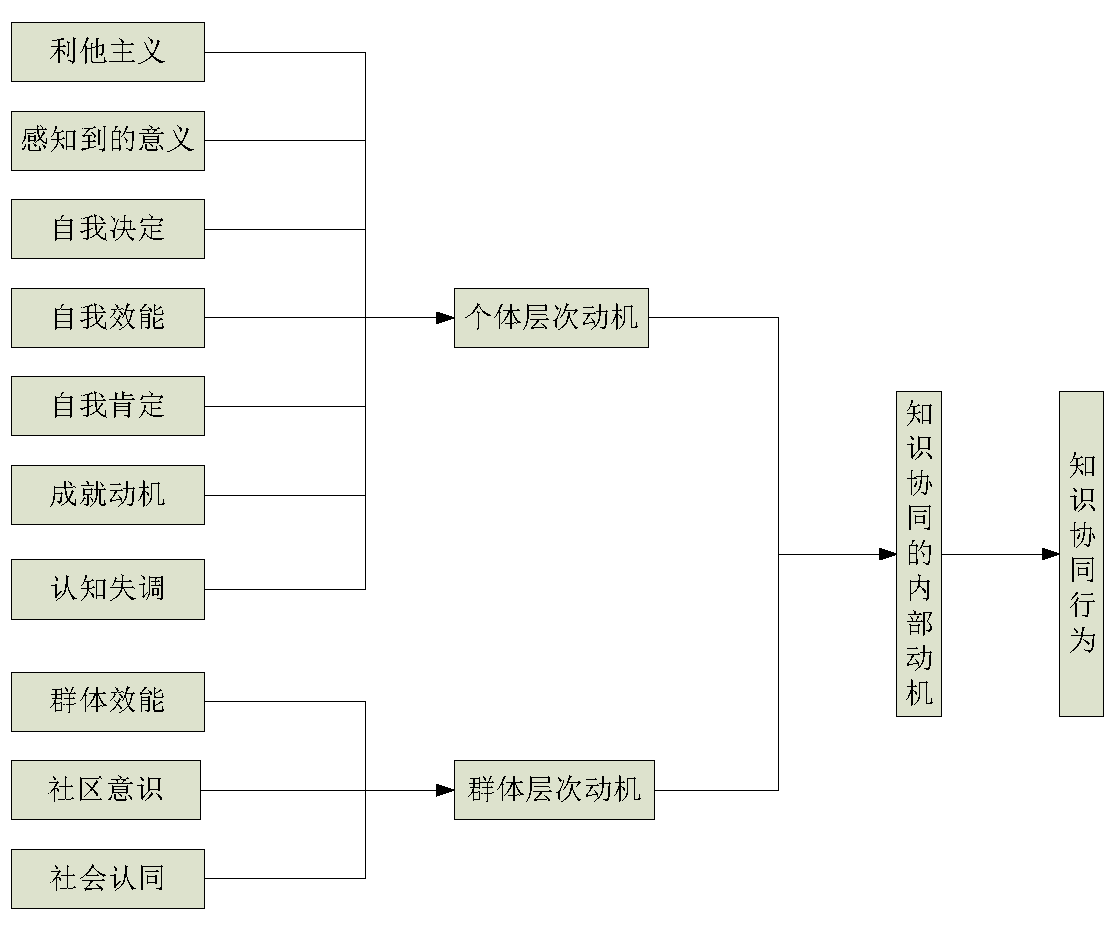
\includegraphics{motivation.pdf}}
    \caption{\small{动机因素与知识协同行为的关系}}
  \label{fig:motivation}
  \end{figure}

Ajzen等提出的理性行为理论认为,个体的行为在某种程度上是可预测的。行为
可以由行为意向推断,行为意向又由个体对行为的态度和主观规范决定。动机是
引起行为的内在原因和动力,因此根据理性行为理论,清楚了个体的动机就可以
去推测个体的行为。上文提到的各种动机因素综合形成了个体参与知识协同的内
部动机。内部动机越强,相应的协同行为水平也就应该越高。通过观察用户参与
知识协同程度的变化,可以进一步发掘动机因素对协同行为的影响。

\subsection{协同行为对动机因素的影响}

尽管动机在一定程度上决定了个体的行为,但是动机并不是静止不变的。随着个
体所处的环境的变化,动机因素也会相应地增强和减弱。特别是在虚拟实践社区
中,人与人的交互非常频繁,外界因素对于个体自身的影响也非常明显。维基百
科社区的用户在参与知识协同的过程中,不断地接收到来此其他协同用户各种类
型的反馈,这种反馈会影响个体自身的动机,尤其是群体层次的动机因素。为
此,有必要详细区分维基百科社区中的各种协同行为,分析协同行为对个体动机
所产生的影响。

在维基百科中,主要的协同行为是编辑条目内容。这些协同行为还可以进一步细
分为:添加内容、删除内容、修改内容。如果从编辑的结果来看可以划分为正向
结果(用户的贡献度为正,条目内容得到改进)和负向结果(用户的贡献度为
负,条目内容质量下降)。具体的协同行为如表\ref{tab:collaboration-activities}所示。
\begin{table}[htb]
  \centering
 \small
  \caption{\small{维基百科中的用户协同行为}}
  \begin{tabular}{|c|c|c|}

\hline
    协同行为&行为描述&协同结果\\\hline
    添加内容&在原有内容基础上新增及内容,同时保持原有内容不受改动。&正
    向改进(+)\\\hline
    添加内容&同上&负向结果(-)\\\hline
    删除内容&删除原文某些内容,同时没有其他内容的变动。&正
    向改进(+)\\\hline
    删除内容&同上&负向结果(-)\\\hline
    修改内容&修改原文中的内容,将不适合或者错误的内容修正&正
    向改进(+)\\\hline
    修改内容&同上&负向结果(-)\\\hline
    新增条目&开设维基百科当前还不存在的条目&正
    向改进(+)\\\hline
    删除条目&由于条目主体不符合维基百科规范而被删除& \\\hline
  \end{tabular}

  \label{tab:collaboration-activities}
\end{table}

除了基本的编辑行为,另有两种行为也纳入到了本文的研究范围:条目的创建和
删除。这是因为条目的创建增加了社区用户参与协同的机会,而删除条目则减少
了用户参与的机会。一些用户的动机会受到这两种行为的影响而产生变化。相对
来讲,个体层次的动机要比群体层次的动机稳定得多,不容易收到外界因素的干
扰;而群体层次的动机本身就产生于个体间的社会化交互,因此更容易收到他人
的反应的影响。

利他主义是人的一种本能表现,是一种客观存在的现象,这已被许多事实所证明。
尽管有人认为并不存在纯粹的利他主义,但是仍然可以看到虚拟实践社区的很多
人确实不求任何回报而愿意为社区做出奉献。利他主义同时是一种很稳定的动机
因素,在维基百科社区已经成为了一种广泛接收的社区氛围。一般不容易受到外
界因素的干扰。因此协同行为对个体的利他主义动机影响很小。

个体所感受到的意义同样是一种稳定的内部动机。这种动机形成于个体参与具体
工作之前最初始的判断。这种判断一旦形成,除非外界环境发生巨大变化,或者
工作本身偏离了其预定目标,否则很难被改变。维基百科的协同用户都认为创建
一个自由的、可任意访问的、包含人类全部知识的在线百科全书是一件了不起的
事情,是一件值得去做的事情。即使自己没有能力做出很大的贡献,或者自己的
投入不能为其他协同用户所承认,都不会妨碍他们对于这件工作自身价值的信念。因此,
感知到的意义受协同行为的影响也很小。

自我决定是个体参与活动自主性的体现。个体的自主性越高,越容易发挥个体自
身的潜力。维基百科为个体提供了足够的自由,个体可以充分感受到自己参与社
区的知
识协同是完全自愿、不带任何强迫成分的。这种自主性是社区本身赋予给每个参与
者的,其他协同者无法剥夺。因此,无论其他协同者有何种协同行为,个体的自主性
都不会受到明显的影响。

自我效能是个体对自身某项能力的信念。这种信念虽然产生于个体自身,但是外
界的反馈会是自我效能发生改变。积极的反馈结果会强化个体的信念,从而增强
其自我效能,而消极的反馈会弱化个体的信念,降低自我效能。知识协同过程中
个体的每一次协同行为都会得到其他人的反馈。这种反馈可以根据本次编辑行为
的贡献度来表示。如果贡献度为正,说明这次编辑受到了其他协同者的认同,个
体对自身能力的信念会强化。如果贡献度为负,则这次编辑的内容未收到其他协
同者的认同,个体对于自身的信念会收到削弱。但是,并非所有的用户对于其他
协同者的反馈反应敏感。对于领导者和领域专家两类用户来说,他们的自我效能
会明显高于其他用户,他们自身及具
有专业的知识和领导能力,同时又对条目的编写具有一定的掌控权。对于其他用户
修改自己的内容这两类用户会根据不同情况持两种态度:1)我坚信我撰写的内容是准确无误的,其
他人修正这些内容是因为他们没有进行仔细的查证和核对;2)我没有同其他用
户进行足够的沟通,未能使他们理解我的编辑意图,在经过协商和讨论后,他们
会接受我的观点。因此,这两类用户的自我效能非常的稳定,不会因为他人的行
为轻易改变。而其他几种类型的用户则不具有这种特点,他们的自我效能容易受
到外界影响。

自我肯定是个体对自身的综合评价。不论是高自我肯定的人还是低自我肯定的
人,都会对其他人的行为做出相应的反应,使得自我肯定的程度发生变化。如果个体的编辑取得了正贡献,对于
高自我肯定的人,这是他人对自身形象的肯定;对于低自我肯定的人,这是个体改变
自身形象所做出的努力得到了他人的肯定。这种情况下,个体的自我肯定都会得
到增强,相应地提升其内部动机。如果个体的编辑取得了负贡献,意味着个体对
于自身形象的信念收到了质疑,但是这并不意味着个体的动机会降低。高自我肯
定的人会投入到其他的编辑中,来弥补这次编辑造成的个人形象的损失;低自我
肯定的人由于没有受到其他人的承认,会更努力地寻找编辑机会来试图提升自己的形象。因
此,不论个体的编辑取得了什么样的结果,个体自我肯定的变化最终都会导致提
升个体的动机。

成就需求是指个体渴望获得成功,或者掌握某种技能等的信念。个体在取得成就
的同时得到心理上的满足。协同行为对于成就动机的影响主要体现为两个方面。
首先,如果个体的编辑受到他人认可,则意味着个体在这次编辑过程中达到了自
己的目的,获得了成功。这种满足感会降低个体的成就需求。其次,如果个体的
编辑未收到认可,而被其他协同者删除或更改,反而会更激发个体的成就需求。
这是因为成就需求动机使人正视所遇到的挫折和失败,并表现出极大的韧性和毅力努
力克服困难和障碍。

当条目的内容于个体自身的信念发生冲突是,就产生了认知失调。不论是其他协
同者编辑的内容有“错误”,还是个体所编辑的内容为他人所修改,都是协同过
程中产生的认知失调。个体面临认知失调时可能采取不同的策略。一种策略是接
收对方的观点,改变自身认知。这表现为那次编辑的贡献为正,既产生失调的内
容为个体所接受,心里的不舒服感觉减弱或者消失,从而参与协同的动机降低。
如果编辑的贡献为负,说明这部分内容并未让个体所接受,个体的失调感继续存
在甚至增强,驱使个体去参与协同过程,将内容修正为符合自己认知的内容。因
此,认知失调相对上述动机因素对于协同行为的反应是正好相反的。认知失调的
特点决定了它不是所有类型用户都适用的动机因素。对于领导者、领域专家和内
容贡献者来说,修正别人的错误不是他们参与协同的主要动机。尽管他们也会在
协同过程中纠正别人的错误,但是他们更多地是把精力投入到拓展条目内容,有
效阻止内容结构上。对于内容维护者和外围用户,认知失调是他们的主要动机因
素之一。这两类用户就是试图发现条目中的错误和漏洞并进行弥补。条目的质量
越高,留给他们参与的机会就越少,他们的参与协同的动机也就越低。

群体效能是个体对于群体能力的感知。这种感知来源于个体所感受到的其他协同者的能
力。如果在某个条目的协同过程中,个体发现其他协同者对于本条目的贡献非常
少,那么他的群体效能感就会下降。在协同过程中,如果其他协同者进行了一次
编辑并取得了正的贡献,则个体会从中感受到他人的力量,群体效能增加,提升
其存于协同的动机。如果个体进行了一次编辑并取得了正的贡献,这就意味着集
体的力量受到了一定程度的削弱,当个体的贡献在整个条目贡献中占据统治地位
时,群体效能则消失殆尽。因此,集体效能只对那些需要借助集体力量意愿较强的个体起
到激励作用,而对集体力量需求较弱的个体作用并不明显。领导者和领域专家这
两类用户通常都是主要依靠自身力量完成条目撰写的。其他人在协同过程中所做
的贡献很小,不能使这两类用户的群体效能发生显著改变。相反的,对于其他三
种类型的用户来说,他们对于集体的力量的感受要强的多,因此协同行为对集体
效能的影响主要体现在这三类用户身上。

社区意识体现了社区中人与人之间的互动联系,以及由此形成的归属感、安定感。
这种感受最终促进了社区的凝聚力,增加了对个体的满意程度,并转化为个体参
与社区活动的动机。当个体的协同行为获得正向反馈时,个体感到自己为社区所
接纳,强化了其作为社区一员的感受;反之如果个体的行为获得了负反馈,个体
会感到自己游离于社区之外,归属感会减弱。同群体效能不同,社区意识不是个
体对群体能力的评价,参与社区同他人交互是人作为社会性动物的基本要求,因
此即使是群体效能较低的人也会拥有较强的社区意识,即与他人沟通交流的需要。
对维基百科中的所有成员来说,如果协同编辑取得正的贡献,则社区意识增加,
协同动机加强,反之社区意识减少,协同动机降低。


\subsection{动机因素之间的相互作用}
\label{sec:interaction}
不仅是协同行为会对动机因素产生影响,动机因素之间也会相互影响。这种相互
作用最终也会引起个体的内部动机的变化,从而影响其协同行为。

自我决定与自我效能。自主性是自我决定的重要特征之一。个体会感到之所以从
事某种活动完全取决于自己的意愿,在这种环境下可以完全发挥个体自身的能力。
这种感受会带来个体自我效能的提升,增强个体的信心。因此,自我决定增强会
引起自我效能的增强。自我效能的增强意味着个体对于自身能力评价的提升,这
会引起个体对于自身胜任能力的提升,个体认为在一个自主的环境下自己可以有
效地处理好各种事情。既自我效能的增强也会自我决定。

自我决定与社区意识。自由地与他人沟通、交互,形成人与人之间的亲密关系是
自我决定的所要满足的需求之一,这与社区意识,尤其是其中的亲和需求在本质上是一
致的,他们是同一事务的两个方面。个体既希望能自由地和他人交往,又希望自
己能为他人所接收。因此自我决定和社区意识形了明显的相互作用。自我决定水
平的提升会引起社区意识的增强,而社区意识的提升也会加强自我决定。

自我决定与归属感。自我决定程度高的个体希望同其他人建立良好的关系。个体
在人际交往中感受到被他人所接纳。而归属感是个体对社区的情感投入。个体感
受到自己是团体中的一分子,愿意为团体的维系和发展做出牺牲。当个体希望参
与社区的意愿越来越强烈使,他会采取一系列的行动促使他人接收自己,而这反
过来又提升了个体的归属感;同样的,对社区有强烈归属感的个体会更愿意与社
区中的人建立密切的关系,从而增强了个体的自我决定感。

成就动机与自我决定。


\section{动机因素的系统动力学模型}
\label{sec:sd-model}
根据上述内容所分析的维基百科社区中用户参与知识协同的各种内部动机可以看
到,形成个体内部动机的原因多种多样,并且互相交织在一起,形成了复杂、动
态的综合动机因素。为了研究个体动机对于协同行为的影响,不但要考虑动机对
于协同的激发作用,还要考虑动机之间的相互关系,以及协同行为的反馈对于动
机的影响。而这使用普通的数学模型是难以进行有效描述的。为了反应动机因素
得这种高阶次、非线性、反馈行和动态性的特点,本文使用系统动力学方法作为
分析建模工具。所建立的模型既要能够进行定量分析,同时还必须容纳一些难于
量化的定性指标,以此来研究动机因素和协同行为之间的因果反馈结构和系统的
动态行为。利用系统动力学方法的有事主要在于:1)可以处理各因素间复杂的
因果关系,全面描述系统的复杂性和动态动态性;2)可以观察到系统长期的演
化过程,对于模型元素的变化所带来的整个系统的改变具有将强的推断能力和预
测能力;3)模型对于数字的精确性要求不高,从而不容易受到微小扰动的干扰,鲁
棒性较强。应用系统动力学模型可以较精确地反应现实世界,为深入地认识和分
析具体的个体的行为模式,提升其参与水平,提出切实有效的管理建议提供可靠
的基础。

\subsection{知识协同的因果回路图}
\label{sec:causality}

为了分析个体的知识协同动机是如何影响知识协同行为的,需要建立各个要素之
间的因果反馈结构,将因果关系清晰地呈现出来。因果回路图是表现系统反馈结
构的重要工具。上文中已经分析了各动机因素和协同行为之间的关系,这些关系
已经在其他的文献和研究中确认为都是明确的因果关系。但是,这种因果关系只
适用于群体均值,而不适用于分析单独的个体。

因果回路图中包含多个变量,这些变量分别是个体的协同行为以及个体的动机因
素,包括个体层面的动机因素和群体层面的动机因素。变量之间存在的因果关系
将变量关联起来,形成因果链。如果因果链之间形成了闭环,就形成了变量间的
反馈回路。每条因果链都有极性。分别用正(+)、负(-)号表示。极性为正意
味着在其他条件不变的情况下,原因的增加将提升结果所能达到的程度。极性为
负意味着在其他条件不变的情况下,原因的增加将降低结果所能达到的程度。

上文分析了影响用户参与知识协同的动机因素。这些动机因素在不同的研究中都
得到了验证,对于用户的参与有很大的影响。但是,已有的研究大部分都不区分
用户类型,而是将所有用户是
为一个整体,认为动机因素对于所有的用户都是同样有效的。但是,通过本文对
用户的分类研究和不同用户的协同模式的分析,这种假设是存在问题的。由于不
同类型的用户具有不同的协同模式,因此并非每一种动机因素都对所有用户其作
用。

在本文所提出的五种类型的用户中,领导者和领域专家这两类用户同其他的用户
有明显的不同。这两类用户在协同过程中表现出极强的自主性和主导型,不轻易
为他人的行为所影响。对于这
两类用户来说,追求编写条目的乐趣以及在编写过程中实现其理想价值才是最重
要的,而参与社交活动,发展人际关系并不是其主要目的\cite{Rafaeli2008}。
因此,群体因素对于这两类用户的影响不大,他们更多的是在个体动机的驱使下
参与到协同活动中的。不论是认知失调、群体效能还是归属感,都不和协同行为
构成显著的因果关系。同时,这两类用户自身的动机比较稳定,不易受到他人行
为的干扰。另外,利他主义对这两类用户的作用也不明显。

对于其他三类用户根据其协同模式可以分析出,这两类用
户即希望从协同活动中满足自身的需求,同时也具有同其他人交互、合作的需求。
因此,本文提出了两个动机因素模型,分别构建其因果回路图,用于分析不同的
用户群体。

领导者和领域专家的因果回路图中包含了8个水平变量,其中7个是动机因素:利
他主义、感知到的意义、自我决定、自我效能、自我肯定以及成就需求。另外一
个水平变量是个体的协同行为。由此形成的因果关系有:1)利他主义精神促使用户参与协同行
为,因果链极性为正;2)感知到的意义促使用户参与协同行
为,因果链极性为正;3)自我决定促使用户参与协同行
为,因果链极性为正;4)自我效能促使用户参与协同行
为,因果链极性为正;5)自我肯定促使用户参与协同行
为,因果链极性为正;6)成就需求促使用户参与协同行
为,因果链极性为正;7)个体的协同行为强化了自我决定,因果链极性为正;8)个体的协同行为
强化了自我效能,因果链极性为正;9)个体的协同行为强化了自我肯定,因果
链极性为正;10)个体的协同行为削弱了成就需求,因果链极性为负;11)自我决定增强
了自我效能,因果链极性为正;12)自我效能能偶促进自我决定意识的增强,因
果链极性为正;13)自我决定能提升个体的成就动机,因果链极性为正。最终所
建立的因果回路图如图\ref{fig:motive1}所示。
\begin{figure}[htb]
  \centering
  \scalebox{0.7}{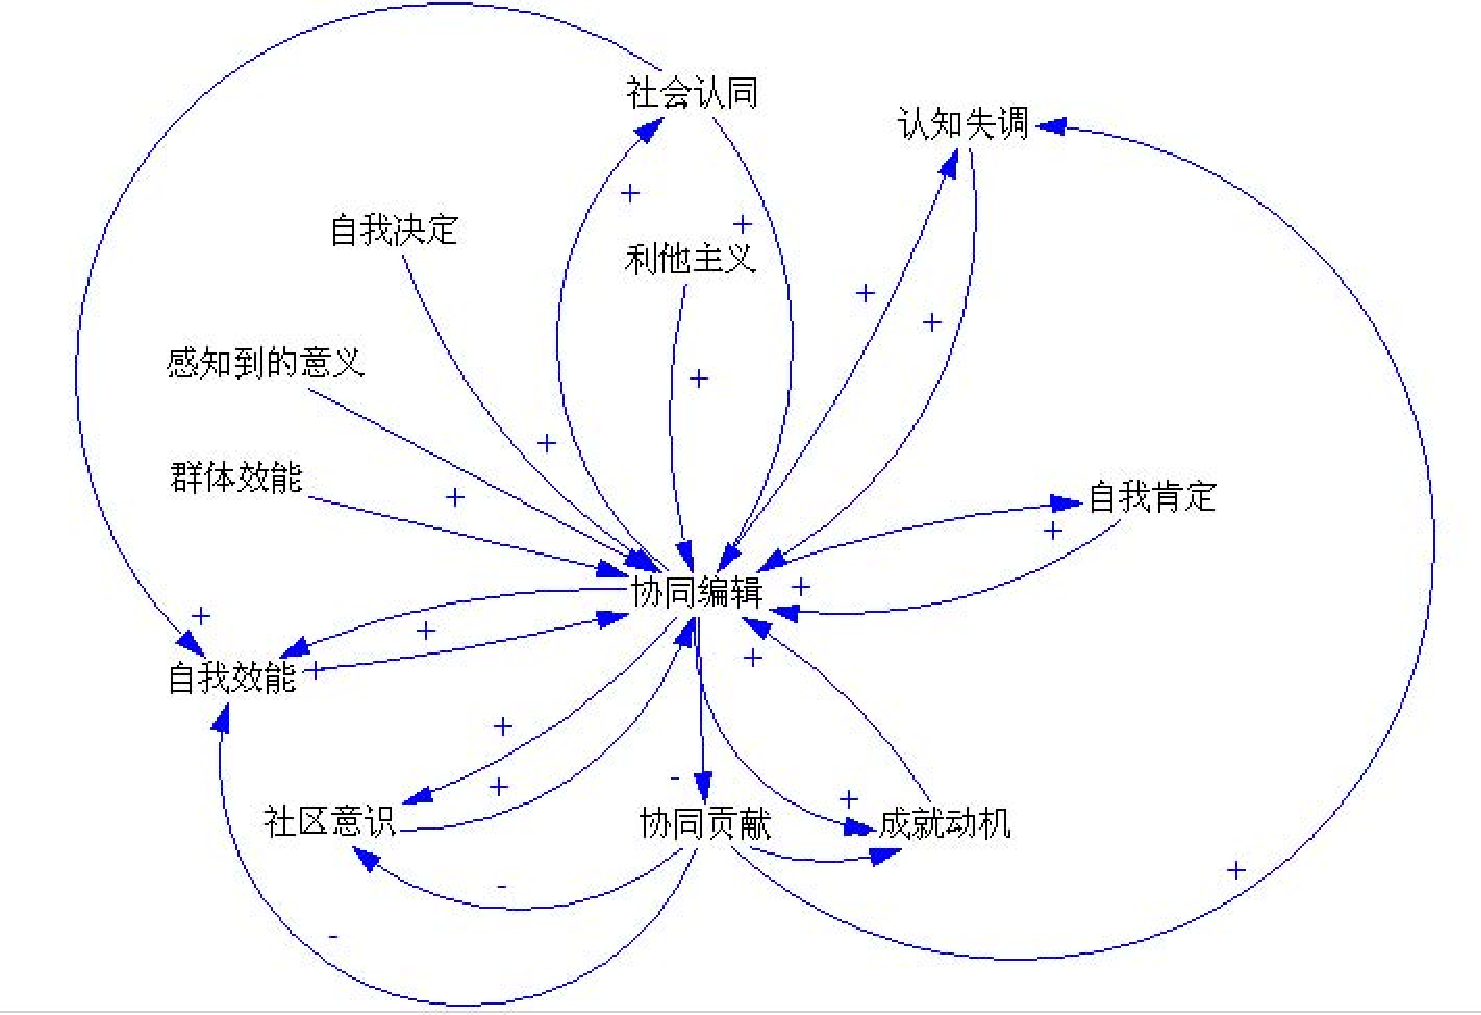
\includegraphics{motive1.pdf}}
  \caption{\small{动机因素模型}}
  \label{fig:motive1}
\end{figure}

内容贡献者、内容维护者以及边缘用户这三类用户占了所有用户的绝大部分。对
于他们来说,在社区中参与社交活动,满足沟通交往的需求同在知识协同过程中获得自我
满足同样重要。因此他们的协同行为同时受到了个体层次的动机和群体层次的动
机的综合影响。人际间的互动对于个体的动机有较大的影响,这几类的用户的行
为容易受到他人行为的干扰。

内容贡献者、内容维护者以及边缘用户这三类用户的因果回路图共包含11个水平
变量。其中9个是动机因素:利
他主义、感知到的意义、自我决定、自我效能、自我肯定、成就需求、群体效能、
认知失调以及归属感。另外两个是用户行为:个体自身的协同行为和他人对个体
的协同行为。其中他人对用个体的协同行为是指其他人修改或删除了个体自身所编
写的内容,既他人对个体的负反馈。由此形成的因果关系有:1)利他主义
促使用户参与行为,因果链极性为正;2)感知到的意义促使用户参与协同行
为,因果链极性为正;3)自我决定促使用户参与协同行
为,因果链极性为正;4)自我效能促使用户参与协同行
为,因果链极性为正;5)自我肯定促使用户参与协同行
为,因果链极性为正;6)成就需求促使用户参与协同行
为,因果链极性为正;7)群体效能促使个体个体参与协同行为,因果链极性为
正;8)认知失调促使个体参与协同行为,因果链极性为正;9)归属感促进个体
参与协同行为;10)个体的协同行为强化了自我决定,因果链极性为正;11)个体的协同行为
强化了自我效能,因果链极性为正;12)个体的协同行为强化了自我肯定,因果
链极性为正;13)个体的协同行为削弱了成就需求,因果链极性为负;14)个体
的协同行为降低了认知失调的程度,因果链极性为负;15)个体的协同行为增强
了个体的归属感;16)个体的协同行为增强了群体效能;17)个体
的协同行为增加了他人对个体的协同行为,因果链极性为正;18)他人对个体的
协同行为降低了个体的自我效能,因果链极性为负;19)他人对个体的协同行为
降低了个体的自我肯定,因果链极性为负;20)他人对个体的协同行为降低了个
体的成就需求动机,因果链极性为负;21)他人对个体的协同行为强化了个体的
认知失调,因果链极性为正;22)他人对个体的协同行为降低了群体效能,因果链极性为负;23)
他人对个体的协同行为降低了个体的归属感,因果链极性为负;24)自我决定增强
了自我效能,因果链极性为正;25)自我效能能偶促进自我决定意识的增强,因
果链极性为正;26)自我决定能提升个体的成就动机,因果链极性为正。27)个
体的归属感提升会使自
我决定增强,因果链极性为正。最终所
建立的因果回路图如图\ref{fig:motive2}所示。

\begin{figure}[htb]
  \centering
  \scalebox{0.7}{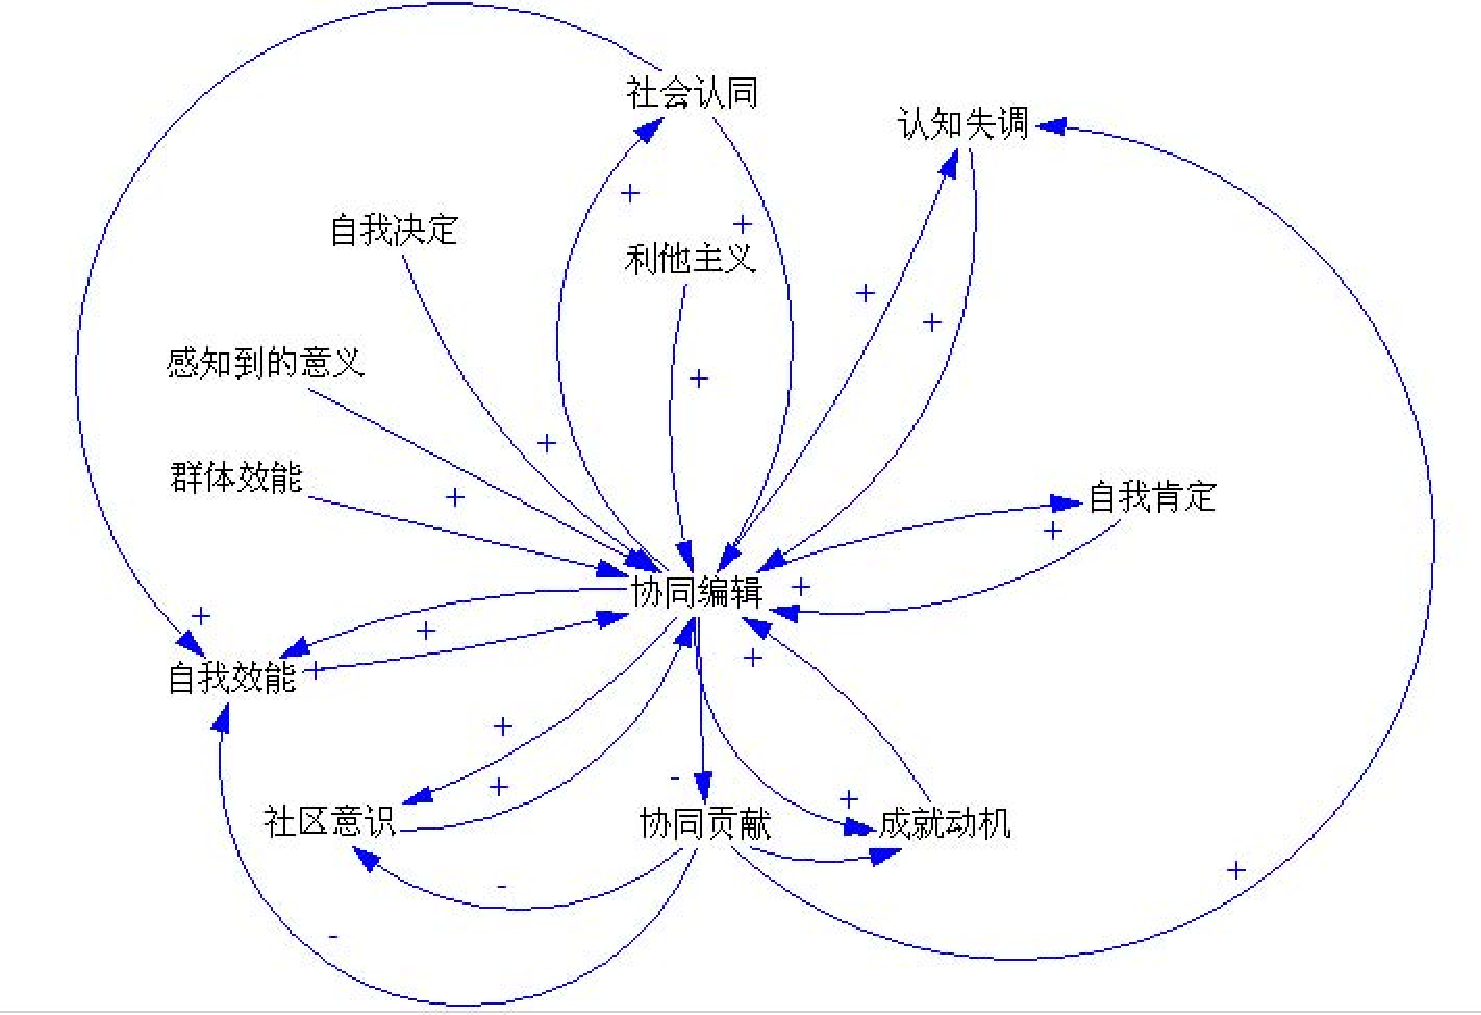
\includegraphics{motive1.pdf}}
  \caption{\small{动机因素模型}}
  \label{fig:motive2}
\end{figure}

\section{本章小结}

本章中分析了影响个体参与知识协同的动机因素,并构建了动机因素与协同行为
间的因果关系模型。动机因素分为两种类型:个体层面的动机因素和群体层面的
动机因素。这两种类型因素的综合作用决定了个体参与知识协同的模式和程度。
同时本章还分析了协同行为对于个体的动机的影响。动机因素会根据行为结果的
反馈增强或者减弱。不但个体自身的行为会影响协同动机,他人的行为也会影响
个体的动机。因此在协同的过程中,个体的动机会不断地发生变化,反过来有影
响其协同行为。另外,动机因素之间也会互相影响,一种动机因素的变化会导致
其他动机产生相应的变化。只有综合考虑因素间的相互影响才能建立有效的动机
模型。

不同类型的用户因为距有不同的协同模式,对其产生影响的动机因素也不尽相同。
对于领导者和领域专家来说,个体层面的动机因素是驱动其参与知识协同的主要
动机;对于其他三类协同者来说,他们既有个人层面的动机,同时也具有群体层
面的动机。因此本文分别建立了两个因果模型来反映不同用户的特点,以供下一步
的进行模型的验证和仿真,具体分析动机对行为的影响。
%%% Local Variables: 
%%% mode: latex
%%% TeX-master: t
%%% End: 
